% Tikz flowchart to show the method used in the pipeline of handling the NGS data.

%block styles for the chart.
\tikzstyle{parent} = [rectangle, draw, fill=red!20, 
minimum width=7.2em, align=center, node distance=1cm, minimum height=1.2em, inner sep=0pt]
\tikzstyle{core} = [rectangle, draw, fill=green!20, 
minimum width=7.2em, align=center, node distance=1cm, minimum height=1.2em, inner sep=0pt]
\tikzstyle{clean} = [rectangle, draw, fill=white, 
minimum width=7.2em, align=center, node distance=1cm, minimum height=1.2em,inner sep=0pt]
\tikzstyle{decide} = [rectangle, draw, fill=yellow, 
minimum width=7.2em, align=center, node distance=1cm, minimum height=1.2em,inner sep=0pt]
\tikzstyle{line} = [draw]
\tikzstyle{arrow} = [thick,->,>=stealth,draw]
%\tikzstyle{dashed} = [thick,dashed,draw]

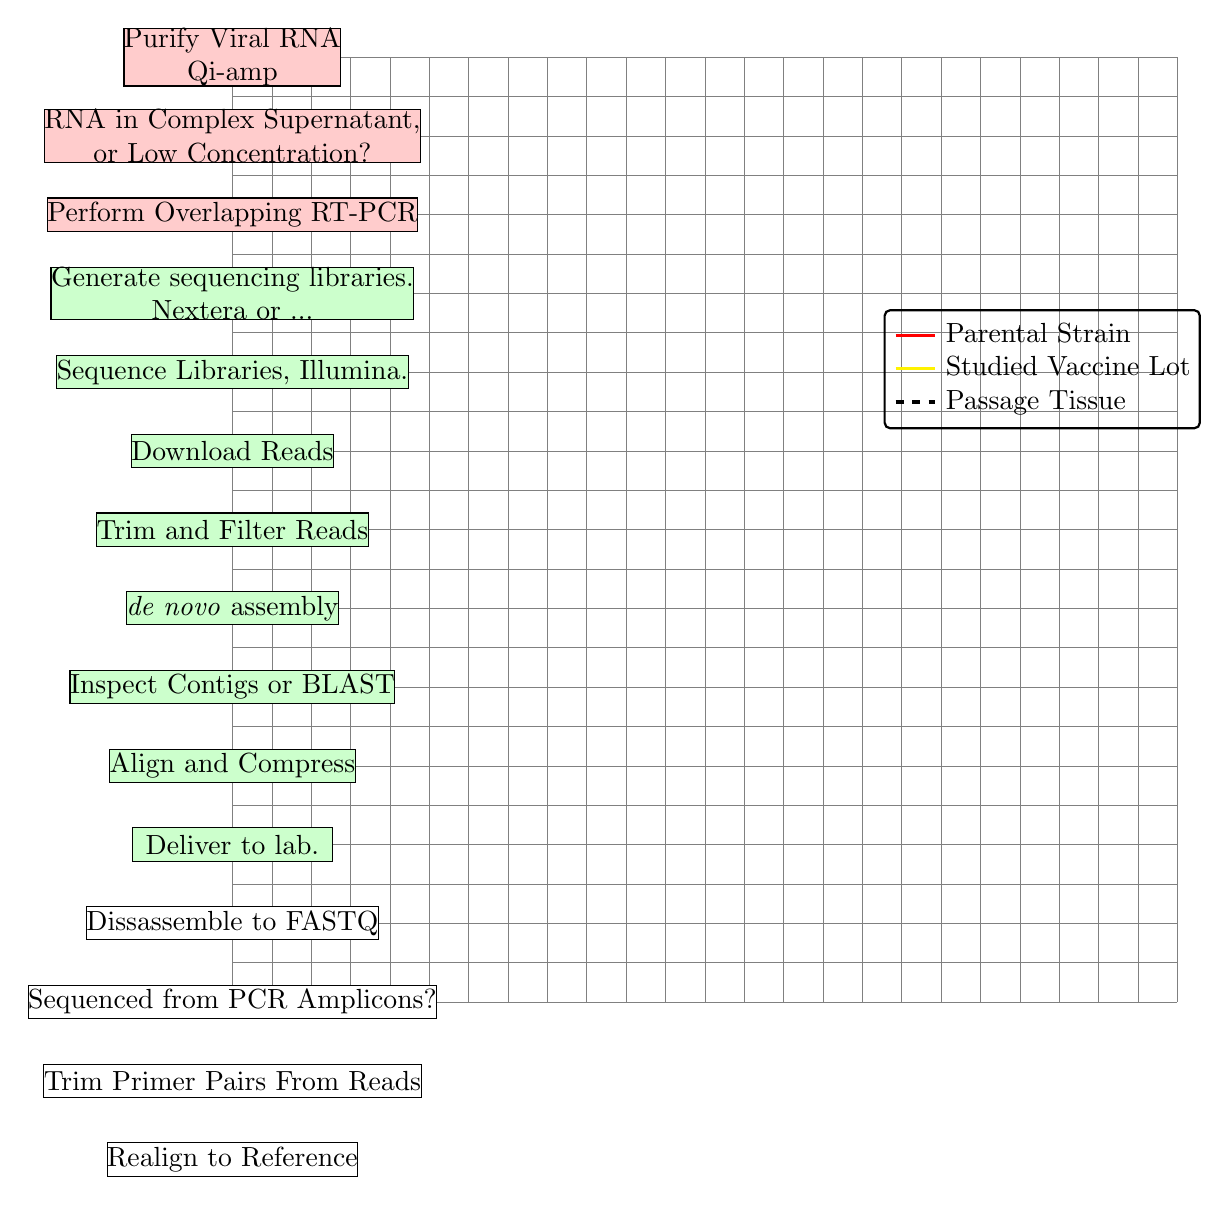
\begin{tikzpicture}[auto]

\draw[help lines,step=.5] (0,0) grid (12,12);

%Nodes for each of the strains mentioned by Yu 2010
% Top
\node[parent](RNA) at (0,12) {Purify Viral RNA \\ Qi-amp};
\node[parent,below of=RNA](isPCR) {RNA in Complex Supernatant,\\ or Low Concentration?};
\node[parent,below of=isPCR](performPCR) {Perform Overlapping RT-PCR};

% Tasks for the Core lab
\node[core, below of=performPCR](library){Generate sequencing libraries.\\Nextera or ...};
\node[core, below of=library](sequence){Sequence Libraries, Illumina.};
\node[core, below of=sequence](download){Download Reads};
\node[core, below of=download](filter){Trim and Filter Reads};
\node[core, below of=filter](assemble){\emph{de novo} assembly};
\node[core, below of=assemble](inspect){Inspect Contigs or BLAST};
\node[core, below of=inspect](align){Align and Compress};
\node[core, below of=align](deliver){Deliver to lab.};

% Tasks after receiving the 
\node[clean, below of=deliver](disassemble){Dissassemble to FASTQ};
\node[clean, below of=disassemble](realign){Sequenced from PCR Amplicons?};
\node[clean, below of=realign](trim){Trim Primer Pairs From Reads};
\node[clean, below of=trim](realign){Realign to Reference};
%
%	
%	%Nodes for each of the three strains considered in the study.
%	\node[studied](TYF2350) at ([xshift=4cm,yshift=-1cm]SA14) {SA14};
%	\node[studied](TYF1454)at ([xshift=4cm,yshift=-0.5cm]SA14-14-2){SA14-14-2};
%	\node[studied, below of=TYF1454](TYF1910){SA14-14-2};	
%	
%	%Arrows connecting the three strains considered in the study.
%	\path[arrow] (SA14-14-2) -| (TYF1454);
%	\path[arrow] (TYF1454) -- (TYF1910);
%	\path[arrow] (SA14) -| (TYF2350);
%	
%	%Arrow connecting Paths
%	\path[arrow] (Mosquito) -- coordinate[midway](M1) (SA14);
%	\path[arrow] (SA14) -- coordinate[midway](M2) (SA14-12-1-7);
%	\path[arrow] (SA14-12-1-7) -- coordinate[midway](M3) (SA14-17-4);
%	\path[arrow] (SA14-17-4) -- coordinate[midway](M4) (SA14-2);
%	\path[arrow] (SA14-2) -- coordinate[midway](M5) (SA14-9);
%	\path[arrow] (SA14-9) -- coordinate[midway](M6) (SA14-9-7);
%	\path[arrow] (SA14-9-7) -- coordinate[midway](M7) (SA14-5-3);
%	\path[arrow] (SA14-5-3) -- coordinate[midway](M8) (SA14-14-2);
%	\path[arrow] (SA14-14-2) -- coordinate[midway](M9) (SA14-14-2-PDK);
%	
%	%Nodes for the passage information
%	\node[information](Mosquito_pass) at ([xshift=-4cm]M1) {11x mb.};
%	\node[information](SA14_pass) at ([xshift=-4cm]M2) {100x PHK, x3 pp. PCE};
%	\node[information](SA14-12-1-7_pass) at ([xshift=-4cm]M3) {2x pp. PCE};
%	\node[information](SA14-17-4_pass) at ([xshift=-4cm]M4) {1x Mouse Spleen(ip.)};
%	\node[information](SA14-2_pass) at ([xshift=-4cm]M5) {3x pp. PCE};
%	\node[information](SA14-9_pass) at ([xshift=-4cm]M6) {1x Mouse Skin};
%	\node[information](SA14-9-7_pass) at ([xshift=-4cm]M7) {6x Hamster Spleen, 2x pp. PHK};
%	\node[information](SA14-5-3_pass) at ([xshift=-4cm]M8) {5x sm. Skin, 2x pp. PHK};
%	\node[information](SA14-14-2_pass) at ([xshift=-4cm]M9) {9x PDK};
%	
%	%Paths connecting passage information nodes with center of arrows.
%	\path[line,dashed] (Mosquito_pass) -- (M1);	
%	\path[line,dashed] (SA14_pass) -- (M2);	
%	\path[line,dashed] (SA14-12-1-7_pass) -- (M3);	
%	\path[line,dashed] (SA14-17-4_pass) -- (M4);
%	\path[line,dashed] (SA14-2_pass) -- (M5);	
%	\path[line,dashed] (SA14-9_pass) -- (M6);	
%	\path[line,dashed] (SA14-9-7_pass) -- (M7);	
%	\path[line,dashed] (SA14-5-3_pass) -- (M8);	
%	\path[line,dashed] (SA14-14-2_pass) -- (M9);	
%	
	
	\node[draw=black,thick,rounded corners=2pt,below left=2mm] at (12.5,9) {%
		\begin{tabular}{@{}r@{ }l@{}}
		%	\raisebox{2pt}{\tikz{\draw[gray, very thick, dashed] (0,0) -- (5mm,0);}}&National Origin\\
		\raisebox{2pt}{\tikz{\draw[red, very thick] (0,0) -- (5mm,0);}}&Parental Strain\\
		\raisebox{2pt}{\tikz{\draw[yellow, very thick] (0,0) -- (5mm,0);}}&Studied Vaccine Lot\\
		\raisebox{2pt}{\tikz{\draw[black,dashed, very thick] (0,0) -- (5mm,0);}}&Passage Tissue\\
		\end{tabular}};	
\end{tikzpicture}